%
% $Id: ch03_thework.tex
%
%   *******************************************************************
%   * SEE THE MAIN FILE "AllegThesis.tex" FOR MORE INFORMATION.       *
%   *******************************************************************
%
\chapter{Method of Approach} \label{ch:method}
In order to create an effective image matching algorithm, it was necessary to pull research, knowledge, and pre-existing code from a number of resources in addition to completing original works. Although the research does not target the hardware infrastructure of the network that image sharing sites use, a simple public web server was built and configured. This topic will be briefly discussed in Section \ref To test the proposed image matching method, it was also necessary to build a skeleton that would act as a simple image sharing website. This skeleton will be capable of accepting an image file and returning a link to the user which will allow the submission to be viewed. The site will also allow for the development of the proposed matching function and will provide the necessary functions to accept and handle the output of the research.

\section{Server Configuration}
In order to implement the website, it is necessary to have an environment capable of running the required processes. To do this, several options were considered. The first option was to run the site on a locally installed Apache web server. After a small amount of testing, this was determined not to be the best option. Due to the lack of a dedicated machine the web server had wildly varying performance due to interference from other processes that could not be closed. This was even a problem when operating on a fixed amount of memory. In addition to this, the XAMPP environment that was tested frequently became momentarily non-responsive with resource hungry processes such as operations performed on large files.

The next alternative was to purchase web space on a shared server. These servers are readily available at minimal cost from dozens of providers such as A Small Orange, BlueHost, and Byethost. After careful consideration several concerns prevented the use of this method. The primary factor was that these servers are shared with numerous users. Due to the nature of this setup, it is unknown how many websites are being hosted by a particular server, and how many concurrent users are accessing these sites at any given time. In addition, it is not possible to set an allotted amount of memory for a particular environment or control what programs are running that may possibly impact the performance of the research.

Another option, that looked very promising at first was to rent server time from a provider such as Amazon Web Services. With this method it is possible to control not only what programs are operational, but it also allows for more freedom of configuration. This would seem like the most probable solution to the problem, but there are still factors that cannot be eliminated such as the speed of the internet connection. By hosting a local web server, it is possible to control this factor, but how much could it affect the results. To test this concern, a server was rented using the free tier services. From this point, a simple timer was configured and one 15 megabyte file was transferred using SFTP. This process was repeated 10 times and the results were analyzed. After reviewing the results, there was no concerning transfer speed variance making this a good match. In the end, it was discovered that there are restrictions to the service that do not allow an individual to alter settings relating to resource allocation, which was a key concern from the start.

The final option was to implement a local dedicated web server and operate the website and scripts from that. The machine proposed would allow not only very tight control over variables such as resource allocation, installed programs, and custom network hardware configuration, but it also allowed usage on a local network or over an internet connection. By running initial tests on a local area network, it is possible to eliminate internet speed fluctuations and control the number of devices utilizing the network bandwidth. This also opened another path where a real world simulation could be run by submitting images to the system over an internet connection and comparing the behavior with only one variable at a time differing.

To build the server a specification had to be determined that would allow optimal performance. To allow the greatest flexibility, the Ubuntu Server operating system was chosen. From this, the server's hardware specifications were chosen based off of the minimum system requirements given by the operating system, Apache suite, and MySQL Database. This information was used to pick a quantity of memory, hard disk space, and processor speed. The server was built with 4 Gigabytes of random access memory (RAM), 3 Gigabytes allocated to the programs and operating system, a 2.43 GHz (Gigahertz) Intel Core i3 processor, and dual 7200 RPM 500 Gigabyte hard drives. The integrated network card was faster than the available network equipment, so it was not of direct concern. The hard disks were chosen to provide ample space for any reasonable number of tests but not provide so much space as to be considered excessive for their purpose. A 7200 RPM variant was also chosen to allow the maximum data throughput and not become a bottleneck when working with great numbers of large image files. Finally, the disks were configured as a redundant mirror to emulate a simple backup system that duplicates the data as a form of backup. This will allow the collection of data and comparison of storage requirement improvements in a non redundant system, and one with a worst case scenario backup implementation that simply creates copies of the files.

The software selection is more straightforward. After selecting to use a Linux operating system, Ubuntu Server was chosen as the distribution. I had the most experience with using, configuring, and troubleshooting issues with this environment and decided it was best for this reason. The accompanying software was fairly simple to select as a quick Google search for "Ubuntu web server" will return thousands of results outlining the setup and configuration of a basic Linux-Apache-MySQL-PHP, or LAMP server. The setup process was completed step by step using the ApacheMySQLPHP LAMP Server Setup Guide provided through the Ubuntu Documentation \cite{ubuntu:lampsetup}. Next, the code which will be discussed shortly requires that the PHP GD Image Library be installed. To prepare the PHP installation to use this library, the server was configured using the direction of the tutorial hosted by nixCraft \cite{nix:gdsetup}.

Upon the completion of the prior configurations, the server was updated and running the latest version of all installed software. To prevent updates from altering the outcomes of the future, a hold was placed on all packages to prevent updates from being installed. In addition to this, the firewall was configured to allow HTTP communication through port 80, which allows interaction through an internet browser with the website hosted on the server. MySQL did not require any setup past the installation of the program and was left alone. At this point, the server configuration was complete and the default Apache "Success" page was displayed when accessing the server showing that everything was working properly.

\section{Website Design}
The core of this research hinges on the successful implementation of an image comparison algorithm. In order to do this, a website needed to be developed that acted in a similar manner to an simple image sharing site. In order to do this, a specific demographic of users had been targeted. Due to the code limitations if the PHP GD Duplicate Image Finder written by CatPa \cite{catpa:gdcode}, only jpeg submissions are accepted for the purpose of this research. In addition to this, a 15 MB file size limit is enforced. This is to prevent excessive wait times when transferring the image file to the server during tests run on a large number of files. The website was designed to be lightweight, more specifically it has no extraneous scripts or applets running on the upload page. The purpose of this is to only give processing times relating to the actual upload process and not unessential scripts. Finally, the last restriction placed on the website development is cross browser compatibility. Instead of placing focus on making a website that functions across all common web browsers, it was decided that a focus on the Geko browsers such as Firefox due to the vast array of development tools available for the browser platform. This limitation will also allow for a focused effort in file management on a specific platform and will allow room for further research after the tool has been optimized.

To begin, a database was implemented in such a way that it holds a vast array of information.


 to hold a hashed key for each uploaded image and the location of the file on the disk in addition to upload statistics to complete the task. An example of this schema can be seen in figure \ref{fig:schema}.

\begin{figure}[htbp]
\centering
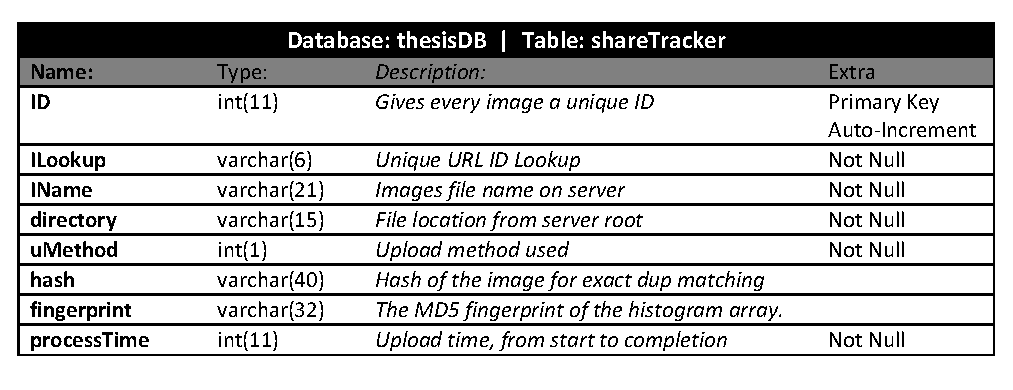
\includegraphics[width=5in]{schema}
\caption{Proposed schema for file uploads}
\label{fig:schema}
\end{figure}

The website will run multiple scripts for each upload. The first script will be a traditional upload method where the user supplies a file, it will be uploaded to the server, and the server will return a unique URL from which to access the image at a later time. During this process, each file will be assigned a new, unique name to prevent collisions upon upload. A SQL {\tt "INSERT"} will then be run on the database for the image and will record the file's location on the server, the file name, the fact it was uploaded using the traditional method, the unique URL to access it from, and an {\tt ID} for each insert into the database. After the completion of the process an {\tt "UPDATE"} will be run on the database entry created by the {\tt "INSERT"} above. The time taken to complete the task will be included in that entry and can be used to analyze the efficiency of both systems upon the completion of the tests outlined in section \ref{sec:evaluate}. This initial upload process can be seen in figure \ref{success_duponly}.

\begin{figure}[htbp]
\centering
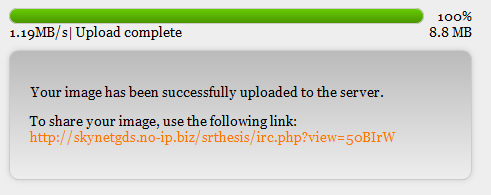
\includegraphics[width=5in]{success_duponly}
\caption{Successful image upload response.}
\label{success_duponly}
\end{figure}

After the first script completes, a second script will be called. The second script has been designed to operate in two steps, the first of which I have already implemented and tested. This function will perform mostly the same task as the traditional upload script, but will check the image being uploaded for duplicates and handle each case appropriately. First, the image will be matched in the most basic form by hashing the image file using an MD5 file hashing function, after which the resulting hash will be compared to all images in the database. Currently this segment of the code has been tested thoroughly and determined to be successfully identifying duplicates and disallowing them in the duplicate-reduced directory. If a match is not found, the script will continue to the second stage of duplicate finding function. For the time being, this second section of the function always returns no duplicate found to enable testing of only the first stage of identification. When this function is implemented in the future, the image will be taken and converted into a $16\times 16$ black-and-white thumbnail and a histogram will be produced from that image. The server will then look into the database and check whether or not any images uploaded with the duplicate reduced system are similar to the one looking to be uploaded. After the calculation is complete, the resulting upload will be accepted by the function and stored on the servers disk. At this time a SQL {\tt "INSERT"} will then be run on the database for the image and will record the files location on the server, the file name, the fact that it was uploaded using the duplicate-reduced method, the unique URL to access it from, the image's MD5 hashed histogram that is described below, and an {\tt ID} for each insert into the database. After the completion of the process an {\tt "UPDATE"} will be run on the database entry created by the {\tt "INSERT"} above. A view of the functioning duplicate-reduced upload process can be seen in figure \ref{success_nodupfound} when no duplicate image is located.

\begin{figure}[htbp]
\centering
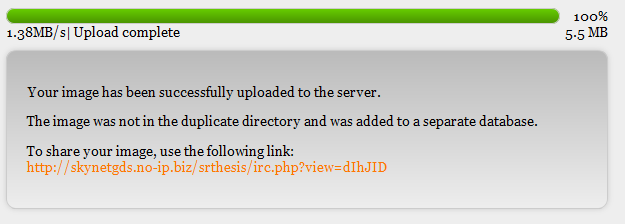
\includegraphics[width=5.5in]{success_nodupfound}
\caption{Successful image upload response when no duplicate is located.}
\label{success_nodupfound}
\end{figure}

If the image histogram hash matches the hash on the server, a color profile will be generated in real time for both images and compared pixel by pixel. If there is a match or close match, the script will compare several small, randomly chosen blocks on the images. If these match, then the image is assumed to be a duplicate and a prompt will be displayed to the user showing them the image they provided and the possible match that already exists. If the image is verified a match, the higher of the two resolutions will be kept, and the user will be given a unique link to the image. If the user decides the image is not a duplicate, the system will run an {\tt "INSERT"} on the database as outlined earlier, and it will be added to the database. Following the completion of this process an {\tt "UPDATE"} will be run on the last {\tt "INSERT"} and the time taken to complete the task will be included in that entry. A view of the functioning duplicate-reduced upload process can be seen in figure \ref{success_dupfound} when a duplicate image is located.

\begin{figure}[htbp]
\centering
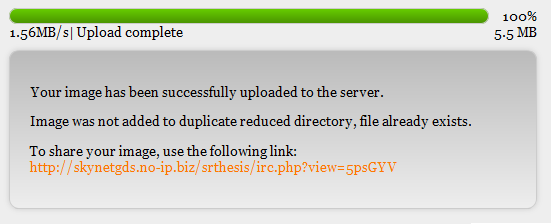
\includegraphics[width=5in]{success_dupfound}
\caption{Successful image upload response when a duplicate is located.}
\label{success_dupfound}
\end{figure}

In the case of requiring duplicate files, where the user decides to upload the image regardless of uniqueness, the script will be able to differentiate between the two images with the unique image ID that is generated at the time of insertion into the database. The closest matching occurrence of an image on the server compared to a new upload will be used in the prompt and displayed to the user. This will prevent frustration with multiple prompts every time more than one duplicate is found.

If an image is indeed found to be duplicate, and the user chooses to use the higher resolution image that is on the server, a unique link will be generated, displayed to the user, and an {\tt "INSERT"} statement will be run containing the same information as the matching file's insert did at the time of upload. This will allow multiple links that point to the same image and the user will be unaware of the system operating in the background which will provide a consistent experience. An outline of this full process can be seen in figure \ref{method-fig1}.

\begin{figure}[htbp]
\centering
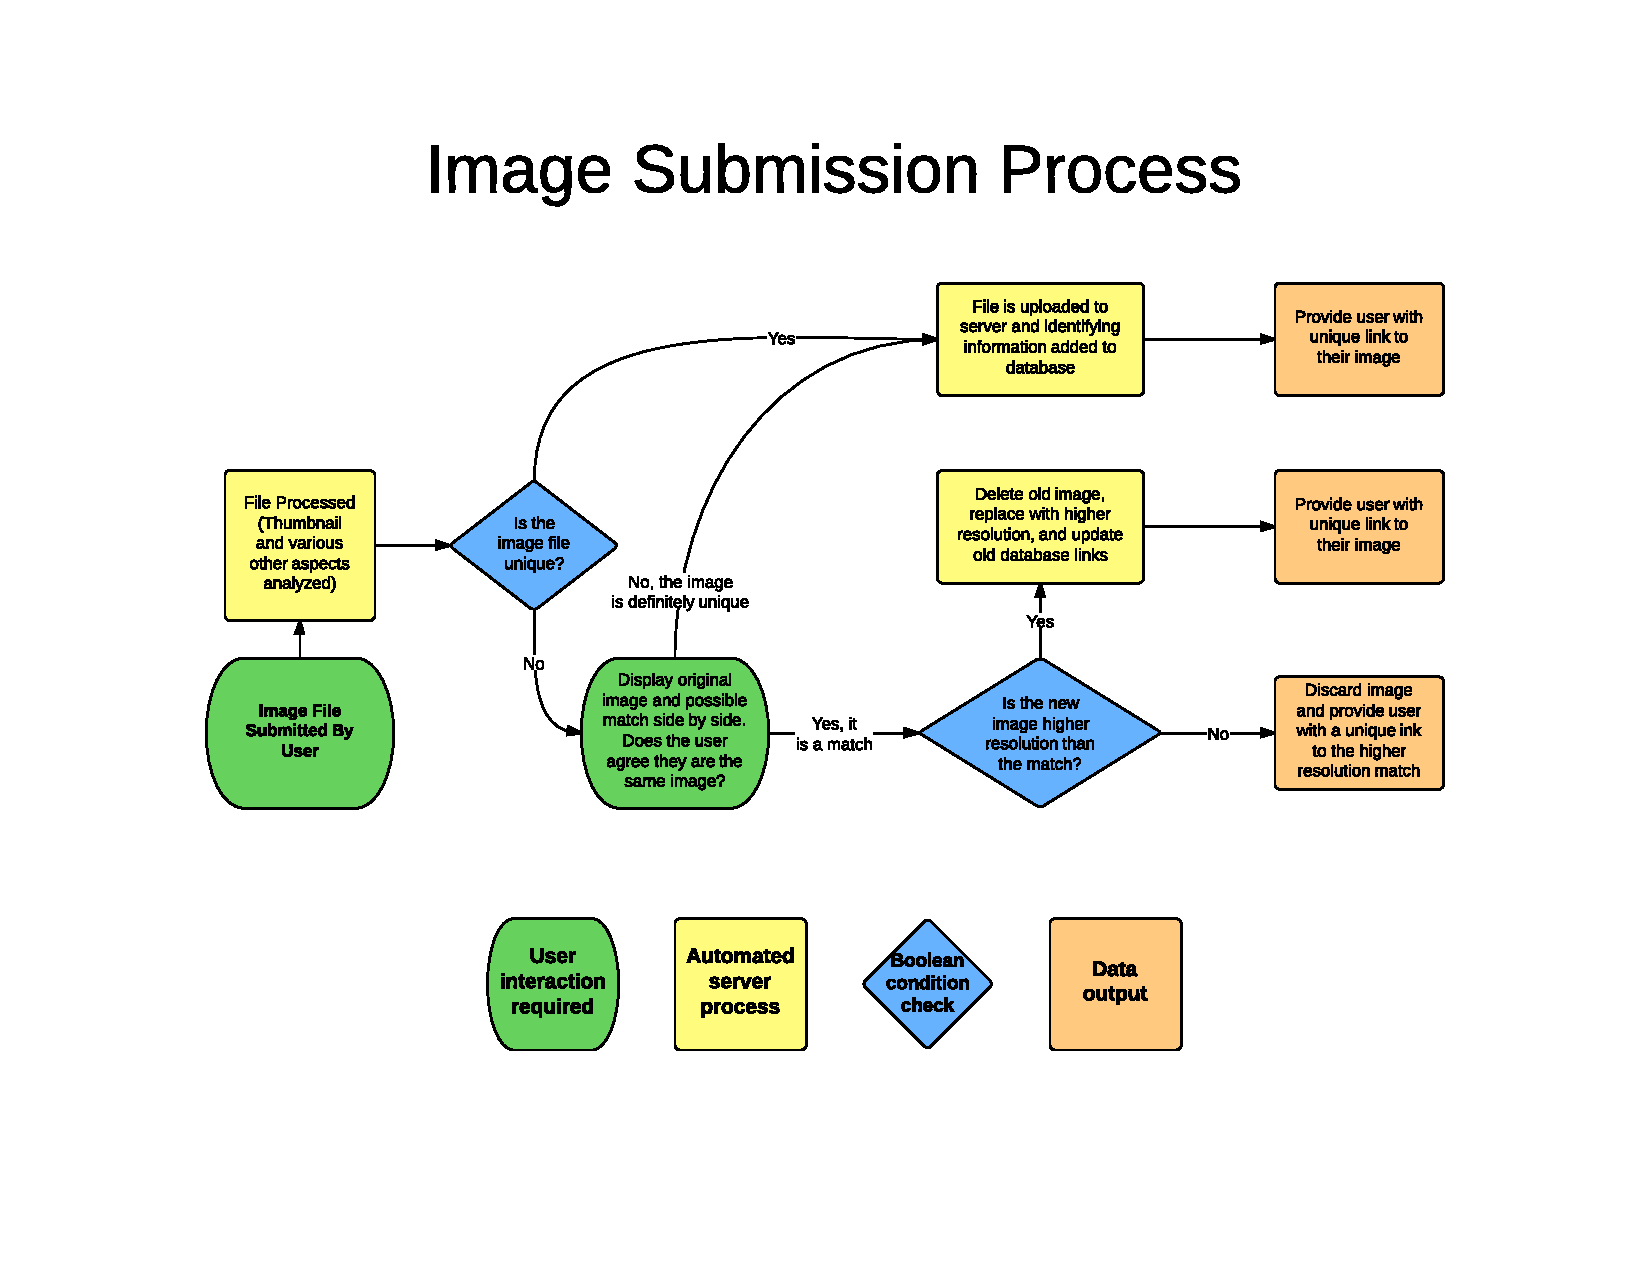
\includegraphics[trim={3cm 3.5cm 2cm 4.2cm},clip, width=6in]{upproc}
\caption{Streamlined upload process}
\label{method-fig1}
\end{figure}

When a user accesses the file from the provided link, the system will run a query that looks up the image identifier provided in the URL. If it matches an image on the server, the image location will be used to provide the image to the user for viewing as seen in figure \ref{viewimage}. The user never notices a difference, but on the server side we have ensured file redundancy has been eliminated and possibly improved user experience by providing the user with higher quality content than what they were expecting. If the requested image is not found, a 404 "Image cannot be found." error will be displayed to let the user know something went wrong.

\begin{figure}[htbp]
\centering
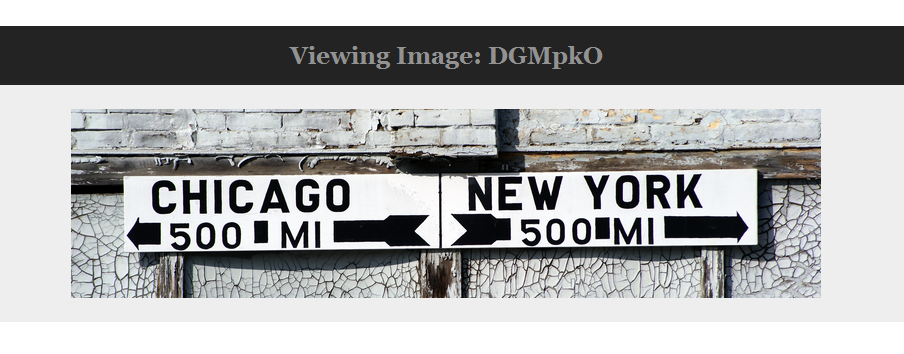
\includegraphics[width=5in]{viewimage}
\caption{What users see when clicking a shared link.}
\label{viewimage}
\end{figure}

\section{Histogram Comparison}
Algorithm \ref{widgmin} (from ) shows a high-level description of an
algorithm. There are many options for the display of
pseudocode; this uses the {\tt algorithm2e} package , 
but there are a number of others available at the Comprehensive \TeX\ Archive
Network (\url{ctan.org}). Using any of these
other packages might require the additon of one or more
``\verb$\usepackage{...}$'' commands in the main {\tt AllegThesis.tex} file.

%   *******************************************************************
%   * SEE CHAPTER ch_01overview.tex FOR INFORMATION ON CONTROLLING    *
%   * PLACEMENT OF FIGURES.                                           *
%   *                                                                 *
%   * THERE ARE MANY DIFFERENT ALGORITHM ENVIRONMENTS. HERE, WE USE   *
%   * THE "algorithm2e" PACKAGE, BUT YOU SHOULD LOOK TO SEE IF        *
%   * OTHER PACKAGES BETTER MEET YOUR NEEDS. REGARDLESS OF WHICH      *
%   * PACKAGE YOU USE, EXPECT TO SPEND TIME READING THE USER MANUAL   *
%   * AS THERE ARE USUALLY A LARGE NUMBER OF PARAMETERS THAT CAN      *
%   * SIGNIFICANTLY AFFECT THE FINAL APPEARANCE OF THE ALGORITHM.     *
%   *******************************************************************

\begin{algorithm}[htbp]
 %\SetLine % For v3.9
 \SetAlgoLined % For previous releases [?]
 \KwData{this text}
 \KwResult{how to write algorithm with \LaTeX2e }
 initialization\;
 \While{not at end of this document}{
  read current\;
  \eIf{understand}{
   go to next section\;
   current section becomes this one\;
   }{
   go back to the beginning of current section\;
  }
 }
 \caption{How to write algorithms (from )}
\label{widgmin}
\end{algorithm}

\section{Experiments}

Figure \ref{javaprog} shows a Java program. There are many, many options for
providing program listings; only a few of the basic ones are shown
in the figure. Some thought must be given to making code suitable
for display in a paper. In particular long lines, tabbed indents, and
several other practices should be avoided. Figure \ref{javaprog} makes
use of the {\tt listings} style file .

%   *******************************************************************
%   * SEE CHAPTER ch_01overview.tex FOR INFORMATION ON CONTROLLING    *
%   * PLACEMENT OF FIGURES.                                           *
%   *                                                                 *
%   * SEE THE MAIN FILE "AllegThesis.tex" FOR THE "\lstset" COMMAND   *
%   * THAT DEFINES HOW PROGRAM LISTINGS WILL LOOK.                    *
%   *                                                                 *
%   * AS WITH EVERYTHING IN LATEX, LOOK AT THE USER MANUAL, SEARCH    *
%   * FOR EXAMPLES ONLINE, CUSTOMIZE TO GET A PLEASING LOOK.          *
%   *******************************************************************


\begin{figure}[htbp]
\centering
\lstinputlisting{Code/SampleProgUncommented.java}
\caption{{\tt SampleProg}: A very simple program}
\label{javaprog}
\end{figure}

\section{Threats to Validity}

